% ═══════════════════════════════════════════════════════════════════════════
\chapter{Datos: captura, reconstrucción y capa canónica}
\label{chap:datos}
% ═══════════════════════════════════════════════════════════════════════════

Los datos de este trabajo no provienen de un proveedor comercial: se capturaron en vivo desde la infraestructura pública de Binance y se reconstruyó con ellos el libro de órdenes completo de BTC/USDT en Binance Spot. Este capítulo describe cómo se hizo y cómo se verificó.

\section{Captura en vivo}
Un servidor dedicado en Alemania se conectó de forma continua a dos flujos públicos de Binance Spot para BTC/USDT: el flujo de profundidad, que publica cada 100~ms los cambios del libro, y el flujo de transacciones, que publica cada operación con su precio, cantidad, lado agresor y hora del motor de negociación. Cada flujo se capturó dos veces en paralelo (captura primaria y de respaldo), de modo que un mensaje perdido por una conexión pudiera recuperarse de la otra. Los archivos se rotaron cada 12 horas y cada mensaje se guardó sin modificar, junto con su hora de recepción local. Periódicamente se descargaron instantáneas completas del libro, que sirven de punto de partida para la reconstrucción.

Las horas registradas permiten medir los retrasos. Binance publica cada transacción alrededor de 1~ms después de ejecutarla. La red añade una mediana de 127--131~ms hasta el servidor (percentiles 5 y 95 de unos 120 y 145~ms). Los mensajes de profundidad llegan en lotes regulares cada 100~ms, sin hora propia para cada cambio dentro del lote.

\section{Reconstrucción del libro}
El libro se reconstruyó siguiendo el procedimiento oficial de Binance para mantener un libro local \citep{BinanceSpotWebSocketDocs}:
\begin{enumerate}[nosep]
\item se parte de una instantánea completa del libro;
\item se aplican los mensajes de profundidad en orden, verificando que sus números de secuencia sean consecutivos;
\item las capturas primaria y de respaldo se combinan por número de secuencia, sin duplicar mensajes;
\item si falta un tramo de secuencia que ninguna captura cubre, el libro se marca como inválido hasta la siguiente instantánea, y ese intervalo nunca se interpola.
\end{enumerate}
Las transacciones se contrastaron con el archivo histórico oficial de Binance, que tiene la hora del motor con resolución de microsegundos; ese archivo se usó para verificar y completar transacciones, nunca para fabricar cambios del libro.

\section{Capa canónica}
A partir del libro reconstruido y de las transacciones se construyó una capa de estado cada 100~ms para el periodo del 29 de junio al 26 de octubre de 2026: 120 días, 864\,000 filas por día y 202 columnas. Cada fila contiene los veinte mejores niveles de cada lado, indicadores de validez y variables causales del libro, del flujo de transacciones y de la volatilidad, calculadas solo con información anterior a la fila. Las 337 millones de transacciones del periodo se conservan por separado, una por una. Toda la capa se construyó con el mismo código, y cada archivo queda registrado en un catálogo que permite verificar su integridad.

La Tabla~\ref{tab:volumen} resume el volumen de datos. El inventario del servidor al 19 de octubre registra 85~GB comprimidos capturados desde el 29 de junio (113 días): 64~GB de libros, 19~GB de transacciones y 2~GB del archivo oficial de Binance. Esa cifra incluye una captura paralela de Coinbase (BTC/USD), que se usó solo en la fase exploratoria. La parte de Binance BTC/USDT, con primaria y respaldo, suma unos 40~GB en esos 113 días. Coincide con lo medido en dos días completos conservados (27 y 28 de julio), que extrapolado a los 120 días da unos 42~GB comprimidos y 430~GB sin comprimir. Cada captura recibió unos 862\,800 mensajes de profundidad al día, de 864\,000 posibles (99,9\,\%), y las dos capturas difieren en pocos cientos de mensajes por día. Unos 880 millones de mensajes crudos se convierten así en una capa de 38~GB lista para modelar.

\begin{table}[htbp]
\centering\small\setlength{\tabcolsep}{4pt}
\caption{Volumen de los datos crudos y de la capa canónica.}
\label{tab:volumen}
\begin{tabular}{@{}lrrr@{}}
\toprule
 & Mensajes o filas & Comprimido & Sin comprimir\\\midrule
Servidor, todo (medido, 113 días) & --- & 85~GB & ---\\
Binance, primaria (120 días) & $\approx$440 millones & $\approx$21~GB & $\approx$214~GB\\
Binance, ambas capturas (120 días) & $\approx$880 millones & $\approx$42~GB & $\approx$430~GB\\
Canónica: libro (202 columnas) & 104 millones de filas & 35~GB & ---\\
Canónica: transacciones & 337 millones & 3~GB & ---\\
\bottomrule
\end{tabular}
\end{table}

\section{Verificaciones}
La Tabla~\ref{tab:auditoria} resume las verificaciones.

\begin{table}[htbp]
\centering\small
\caption{Verificaciones de la reconstrucción y de la capa canónica.}
\label{tab:auditoria}
\begin{tabular}{@{}p{.70\textwidth}r@{}}
\toprule Verificación & Resultado\\\midrule
Tramos entre instantáneas cuyo libro reconstruido coincide exactamente con la instantánea siguiente (100 niveles por lado) & 103 de 116\\
Instantáneas posteriores con fila correspondiente que coinciden exactamente en 20 niveles & 18 de 18\\
Conflictos de precio o cantidad entre transacciones capturadas y el archivo oficial & 0\\
Mejores precios distintos frente a una reconstrucción independiente (22,9 millones de filas comparadas) & 2 por lado\\
Libros cruzados, niveles desordenados o cantidades no positivas & 0\\
Fracción mínima de filas válidas en un día & 99,95\,\%\\
Tiempo con spread de un tick (0,01~USDT), entrenamiento & 99,96\,\%\\
\bottomrule
\end{tabular}
\end{table}

Los 13 tramos que no coinciden contienen huecos de secuencia; quedaron marcados como inválidos y no se usaron. Las pequeñas diferencias de profundidad frente a la reconstrucción independiente (0,01--0,04\,\% de las filas) se concentran en niveles alejados del mejor precio.

\section{Causalidad y alineación de relojes}
\label{sec:datos-resultados}

Las covariables deben usar solo información anterior a cada decisión. Para comprobar que la capa no contiene información del intervalo que se quiere predecir se midió, para cada transacción agresiva que barre varios niveles, la fracción de casos en que el libro vigente $s$ milisegundos después del evento ya refleja el barrido. Si hubiera fuga, el barrido aparecería en $s\le0$. La fracción se mantiene en el nivel de fondo (cerca de 1\,\%) hasta $s=80$~ms, sube desde $s\approx90$~ms y se completa hacia $s\approx200$~ms (Figura~\ref{fig:reloj}).

\begin{figure}[htbp]
\centering
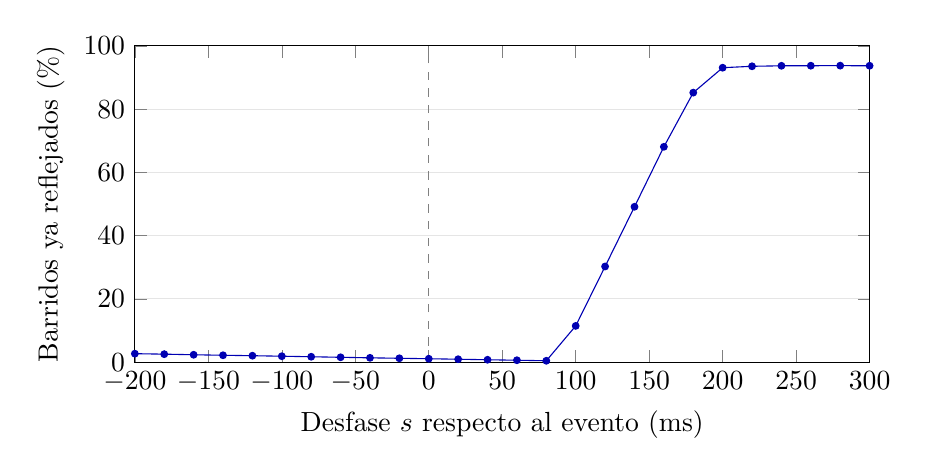
\begin{tikzpicture}
\begin{axis}[width=.9\textwidth,height=5.6cm,xlabel={Desfase $s$ respecto al evento (ms)},ylabel={Barridos ya reflejados (\%)},
 xmin=-200,xmax=300,ymin=0,ymax=100,ymajorgrids=true,grid style={gray!20},mark size=1.2pt]
\addplot[blue!70!black,mark=*] coordinates {(-200,2.70) (-180,2.55) (-160,2.36) (-140,2.20) (-120,2.06) (-100,1.90) (-80,1.73) (-60,1.56) (-40,1.39) (-20,1.25) (0,1.10) (20,0.95) (40,0.78) (60,0.63) (80,0.46) (100,11.48) (120,30.26) (140,49.13) (160,68.08) (180,85.20) (200,93.08) (220,93.53) (240,93.68) (260,93.71) (280,93.73) (300,93.69)};
\draw[dashed,gray] (axis cs:0,0) -- (axis cs:0,100);
\end{axis}
\end{tikzpicture}
\caption{Fracción de barridos multinivel ya reflejados en el libro $s$ milisegundos después del evento, 29 de junio de 2026 (155\,676 barridos). Otros días muestran el mismo patrón.}
\label{fig:reloj}
\end{figure}

No hay fuga detectable: el libro va unos 90~ms detrás del reloj de las transacciones, por la publicación en lotes de 100~ms. Un participante real vería además el estado con el retraso de red. Por eso se verificó, con la versión original de E3, que un retraso adicional de 200~ms en las covariables conserva entre el 81 y el 90\,\% de su ventaja predictiva.
